\documentclass[pdftex,a4paper,12pt]{report}

\usepackage[linesnumbered,boxruled,vlined]{algorithm2e}
\usepackage{amsmath}
\usepackage{hyperref}
\usepackage{color}
\usepackage{fullpage}
\usepackage{graphicx}
\renewcommand{\thesection}{\arabic{section}}

\hypersetup{
  colorlinks,
  citecolor=blue,
  linkcolor=blue,
  urlcolor=blue
}
\begin{document}
\begin{titlepage}
\begin{center}

\textsc{\LARGE IIT Kanpur}\\[1.5cm]

\textsc{\Large CS345A - AlgorithmsII}\\[0.5cm]

% Title
{ \huge \bfseries Assignment 2 \\[0.4cm] }


\begin{minipage}{0.4\textwidth}
\begin{flushleft} \large
Anjani Kumar\\
11101
\end{flushleft}
\end{minipage}
\begin{minipage}{0.4\textwidth}
\begin{flushright} \large
Sumedh Masulkar\\
11736
\end{flushright}
\end{minipage}

\vfill

% Bottom of the page
{\large January 22, 2014}

\end{center}
\end{titlepage}

\tableofcontents
\newpage
\section{Multi-Swap in dynamic sequence}

\paragraph{Overview} \mbox{}\\

The data structure used for saving the sequence will be an augmented red black(height balanced) binary tree. 
The design of the tree would be such that inorder traversal of the tree anytime would output the sequence.\\

The data structure will perform the following operations, all in $O(log\ n)$:
\begin{itemize}
	\item Insert($D, i, x$).
	\item Delete($D, i$).
	\item Multi-Swap($D, i, j$).
	\item Report($D, i$).
\end{itemize}

Augmentation of binary tree (Every node will store these keys in addition to the standard keys kept in nodes of a 
red-black binary tree):
\begin{itemize}
	\item \textbf{flip bit:} This variable will act as a flag to tell whether the subtree
	 of this node are to be flipped or not. If $flip$ is 1, this means the subtrees of this node are flipped,
	 $i.e.$ left child anywhere in the subtrees of this node will actually be the right child, and similarly 
	 the right child will be the left child of its parent. If $flip$ is 0, then the relationship between the parent and 
	 children nodes will be normal(as always).
	
	\item \textbf{size:} This variable stores the size of a subtree at a given node. The size of the subtree means 
	numbers of nodes in the subtree. Hence, size at a given node will be (1 + size of left subtree + size of right subtree).
	
	\item Other standard fields:
		\begin{itemize}
			\item val(u): value of the node.
			\item left(u): pointer to left child of the node.
			\item right(u): pointer to right child of the node.
			\item parent(u): pointer to parent of the node.
			\item color(u): color of the node.
		\end{itemize}
\end{itemize}
\newpage
\subsection{Insert($D, i, x$)}
\paragraph{} Insert an element $x$ at $i^{th}$ position in the sequence.
\paragraph{} 
Insert operation in this data structure will be according to the size variable and flip bits.
Traversal of the tree during insertion will be according to the flip bit. If number of flips encountered 
in the way are odd, then the left and right child will have to be considered as reversed, if number of flips are
even, then we will traverse normally. This means if a node has to be flipped, its left child will be considered as 
right, and vice versa.\\\\
Position of insertion will be found according to the size variable.\\
Suppose, we are at a node $u$. Let s be the size of left subtree of $u$, and $i$ is the position where $x$ is to be 
inserted. If $i\ \leq\ s+1$, then $x$ should be inserted in left subtree of $u$. Otherwise, if $i\ >\ s$, 
then $x$ will be inserted in the right subtree of $u$.

\paragraph{Time Complexity:} \makebox[2pt]{}\\
For any insertion, we will be traversing from root to leaf, thus taking $O(h)$ time. Hence, time complexity for this operation will
be $O(log\ n)$.
\begin{algorithm}
Initialize flips$\gets$ 0;\makebox[40pt]{}\textcolor{blue}{//this variable flips is global, where flip(T) refers to
 flip \makebox[150pt]{} //bit of that node.}\\
Insert($T$, $i$, $x$)\{\\
\Begin{
	flips $\gets$ (flips + flip($T$))\%2\;
	size($T$)$\gets$size($T$)+1\;     		
      \uIf{$T$==\textcolor{red}{NULL}}{
 			create a new node $u$\;
 			val($u$)$\gets x$; flip($u$)$\gets$0\;
 			left($u$)$\gets$\textcolor{red}{NULL}; right($u$)$\gets$\textcolor{red}{NULL}\;
 			return $u$\;
      }
      \uElseIf{flips==0}{
      		\eIf{left($T$)==\textcolor{red}{NULL}}{
     			s$\gets$0\;
     		}{
     			s$\gets$ size(left($T$))\;
     		}
     		\eIf{$i\ \leq\ s+1$}{
     			left($T$)$\gets$ Insert(left($T$), $i$, $x$)\;
     		}{
     			right($T$)$\gets$ Insert(right($T$), $i-s-1$, $x$)\;
     		}
     		return $T$\;
      }
      \uElse{\makebox[40pt]{}\textcolor{blue}{//flip is 1.}\\
			\eIf{right($T$)==\textcolor{red}{NULL}}{
     			s$\gets$0\;
     		}{
     			s$\gets$ size(right($T$))\;
     		}
     		\eIf{$i\ \leq\ s+1$}{
     			right($T$)$\gets$ Insert(right($T$), $i$, $x$)\;
     		}{
     			left($T$)$\gets$ Insert(left($T$), $i-s-1$, $x$)\;
     		}
     		return $T$\;
      }
}     
\}\\
\caption{Pseudo code for insert operation}
\end{algorithm}

\newpage
\subsection{Delete($D, i$)}
\paragraph{} Delete $i^{th}$ element from the sequence.\\\\
Delete operation also will be similar to Insert() operation.\\
The flip bits along the path if even, then traversal will be normal else if number of flips 
encountered are odd, the right child will actually be the left child and vice-versa. 
The $i^{th}$ element will be found similarly with the help of the size variables stored in the nodes.
\begin{itemize}
	\item \textbf{Remove():} Function Remove() will be used as a black box in Delete() Operation. This Remove() function
	is the standard deletion of a node in a Red-Black tree, $i.e.$ the node will be removed and height balancing will be 
	done as usual. The size fields and flip bits will also be updated accordingly. This operation has time complexity 
	$O(log\ n)$.
\end{itemize}

\paragraph{Time Complexity:} \makebox[2pt]{}\\
For any deletion, we will be traversing from root to leaf, thus taking $O(d)$ time, where $d$ is depth of tree. Then, Remove()
which is normal deletion in a red-black tree has time complexity $O(log\ n)$. Hence, time complexity for this operation will
be $O(log\ n)$.
\begin{algorithm}
Initialize flips$\gets$ 0;\makebox[40pt]{}\textcolor{blue}{//this variable flips is global, where flip(T) refers to
 flip \makebox[150pt]{}//bit of that node.}\\
Delete($T$, $i$)\{\\
\Begin{
	flips $\gets$ (flips + flip($T$))\%2\;
	size($T$)$\gets$size($T$) - 1\;
	      \eIf{flips==0}{
      		\eIf{left($T$)==\textcolor{red}{NULL}}{
     			s$\gets$0\;
     		}{
     			s$\gets$ size(left($T$))\;
     		}
     		\uIf{$i\ <\ s+1$}{
     			left($T$)$\gets$ Delete(left($T$), $i$, $x$)\;
     		}
     		\uElseIf{$i\ >\ s+1$}{
     			right($T$)$\gets$ Delete(right($T$), $i-s-1$, $x$)\;
     		}
     		\uElse{
     			Remove($T$);
     		}
     		return $T$\;
      }{\makebox[40pt]{}\textcolor{blue}{//flip is 1.}\\
		\eIf{right($T$)==\textcolor{red}{NULL}}{
     			s$\gets$0\;
     		}{
     			s$\gets$ size(right($T$))\;
     		}
     		\uIf{$i\ <\ s+1$}{
     			right($T$)$\gets$ Delete(right($T$), $i$, $x$)\;
     		}
     		\uElseIf{$i\ >\ s+1$}{
     			left($T$)$\gets$ Delete(left($T$), $i-s-1$, $x$)\;
     		}
     		\uElse{
     			Remove($T$)\;
     		}
     		return $T$\;
      }
}     
\}\\
\caption{Pseudo code for Delete operation}
\end{algorithm}

\newpage
\subsection{Report($D, i$):} 
\paragraph{} Report $i^{th}$ element from the sequence.\\\\
Traversal will be similar to Insert() and Delete() operations.\\
If flip is 1, consider tree to be flipped. Else traverse normally.\\
And for selecting the direction, check the size of left subtree. If size is smaller than $i$, go to 
right subtree, else traverse left subtree.\\\\

\paragraph{Time Complexity:} \makebox[2pt]{}\\
For any report, we will be traversing from root to leaf, thus taking $O(h)$ time. Hence, time complexity for this operation will
be $O(log\ n)$.
\begin{algorithm}
Initialize flips$\gets$ 0;\makebox[40pt]{}\textcolor{blue}{//this variable flips is global, where flip(T) refers to
 flip \makebox[150pt]{}//bit of that node.}\\
Report($T$, $i$)\{\\
		found$\gets$false; $u\gets T$\;
		\While{\textcolor{red}{not} found}{
			flips $\gets$ (flips + flip($T$))\%2\;
			\eIf{flips==0}{
				\eIf{left(u)==\textcolor{red}{NULL}}{
					s$\gets$0\;
				}{
					s$\gets$size(left($u$))\;
				}
				\uIf{s== $i$-1}{
					found$\gets$true\;
				}
				\uElseIf{s$\ >\ i$-1}{
					$u\gets$ left($u$)\;
				}
				\uElse{
					$u\gets$ right($u$)\;
					$i\gets$ $i$ -s -1\;
				}
			}{
				\eIf{right($u$)==\textcolor{red}{NULL}}{
					s$\gets$0\;
				}{
					s$\gets$size(right($u$))\;
				}
				\uIf{s== $i$-1}{
					found$\gets$true\;
				}
				\uElseIf{s$>\ i$-1}{
					$u\gets$ right($u$)\;
				}
				\uElse{
					$u\gets$ left($u$)\;
					$i\gets$ $i$ -s -1\;
				}
			}
		}
		return val($u$)\;
\}\\
\caption{Pseudo code for Report operation}
\end{algorithm}


\newpage
\subsection{MultiSwap($D, i, j$)}
\paragraph{} Swap all elements from $ i^{th} $ place to $ j^{th} $ place. For example, if the sequence is
(x, a, e, b, f, h, z, d). Then, after MultiSwap(D, 3, 7), the sequence becomes (x, a, z, h, f, b, e, d).

\paragraph{}
The algorithm for MultiSwap() uses two other following operations as black boxes:
\begin{enumerate}

	\item \textbf{Merge($T_1$, $T_2$):} Given two trees $T_1$ and $T_2$ having the same height h, we can find an element x
	and the added constraint that all elements of $T_1$ are smaller than x, and all elements of $T_2$ are larger than x, merge these into 
	a single red-black tree. This operation can be done in $O(log\ n)$ time, as we have seen earlier in CS210 course.

	\item \textbf{Split($T$, $x$):} This operation is just the opposite of Merge() described above. The aim is to split 
	T into two red-black trees $T_1$ and $T_2$ such that $T_1$ stores all the elements of $T$ which are smaller 
	than $x$ and $T_2$ stores elements of $T$ greater than $x$. Using $O(log\ n)$ time algorithm for Merge() just 
	as a black box, it is possible to perform Split($T$, $x$) in $O(log\ n)$ time, as was implemented in CS210.
	
	\item \textbf{Height($T$):} Returns black height of the tree rooted at $T$. Takes $O(log\ n)$ since black height from 
	root to any leaf will be same as any other. Thus, this would be as simple as going to the left of node, while left
	node is null and incrementing height variable.
\end{enumerate}

\paragraph{What needs to be done for MultiSwap($T, i, j$)?}
\begin{enumerate}
	\item Let T be the tree which stores sequence S. Note that inorder traversal of this tree gives sequence S.
	We will have to keep in mind the flip bits stored at various nodes to get the correct sequence from $T$.
	\item Split the tree $T$ into $T_1$ and $T'$ such that $T_1$ stores the first $i$-1 elements, and $T'$
	stores the rest.
	\item Split $T'$ further into $T_2$ and $T_3$, such that $T_2$ stores next $j$-$i$+1 elements of the sequence 
	after elements in $T_1$.
	\item The operations till now have been such that all the elements to be swapped are contained in $T_2$.
	\item Reverse flip bit of root of $T_2$,$i.e.$ flip($T_2$)$\gets \textcolor{red}{not}$(flip($T_2$)).
	\item Merge $T_1$ with $T_2$ to get $T'$, and then $T_3$ with $T'$ to get $T$. Thus, the sequence has
	been swapped.
	\item Note that for each operation of split and merge, we need to take care of flip bit stored in respective 
	nodes (or roots). It takes $O(log\ n)$ time to split a height balanced trees around any element and $O(log\ n)$ 
	time for merging two height balanced trees of combined size n.
	\item \underline{Point to note:} While Merging, if black height of $T_1$ is greater than that of $T_2$, then root of $T_2$ 
	will be successor of root of $T_1$, hence $T_1$ doesn't need to be flipped. But if black height of $T_2$ is greater, 
	then $T_1$ will be successor of $T_2$, now since $T_2$ is flipped, $T_1$ will also get flipped. To avoid this, we should 
	also flip $T_1$. Thus resetting flip for nodes in $T_1$. Similar method should be adopted while merging T' and $T_3$.
\end{enumerate}

\begin{algorithm}
MultiSwap($D$, $i$, $j$)\{\\
\Begin{
	$x$ $\gets$ Report($T$, $i$); \makebox[70pt]{}\textcolor{blue}{//$O(log\ n)$}\\
	$T_1$, $T'$ $\gets$ Split($T$, $x$);	\makebox[60pt]{}\textcolor{blue}{//$O(log\ n)$}\\
	$y$ $\gets$ Report($T'$, $j-i+1$);	\makebox[40pt]{}\textcolor{blue}{//$O(log\ n)$}\\
	$T_2$, $T_3$ $\gets$ Split($T'$, $y$);\makebox[60pt]{}\textcolor{blue}{//$O(log\ n)$}\\
	flip($T_2$) $\gets$ \textcolor{red}{not}(flip($T_2$));\makebox[40pt]{}\textcolor{blue}{//where not(0)=1, not(1)=0.}\\
	$h_1$ $\gets$ Height($T_1$);		\makebox[70pt]{}\textcolor{blue}{//$O(log\ n)$}\\
	$h_2$ $\gets$ Height($T_2$);		\makebox[70pt]{}\textcolor{blue}{//$O(log\ n)$}\\
	$h_3$ $\gets$ Height($T_3$);		\makebox[70pt]{}\textcolor{blue}{//$O(log\ n)$}\\
	\eIf{$h_1 > h_2$}{
		$T'\ \gets$ Merge($T_1,\ T_2$);	\makebox[40pt]{}\textcolor{blue}{//$O(log\ n)$}\\
	}{
		flip($T_1$) $\gets$ \textcolor{red}{not}(flip($T_2$))\;
		$T'\ \gets$ Merge($T_1,\ T_2$);	\makebox[40pt]{}\textcolor{blue}{//$O(log\ n)$}\\
	}
	$h \ \gets$ Height($T'$);			\makebox[70pt]{}\textcolor{blue}{//$O(log\ n)$}\\
	\eIf{$h < h_3$}{
		$T\ \gets$ Merge($T',\ T_3$);		\makebox[40pt]{}\textcolor{blue}{//$O(log\ n)$}\\
	}{
		flip($T_3$) $\gets$ \textcolor{red}{not}(flip($T_3$))\;
		$T\ \gets$ Merge($T',\ T_3$);		\makebox[40pt]{}\textcolor{blue}{//$O(log\ n)$}\\
	}
	return $T$;
}
\}\\

\caption{Pseudo-code for MultiSwap operation}
\end{algorithm}

\paragraph{Time Complexity:} \makebox[2pt]{}\\
As can be seen in the algorithm, all steps have maximum $O(log\ n)$, and each step is carried out only once. Thus, 
time complexity of the operation is $O(log\ n)$.


\newpage

\section{Point of Maximum Overlap: A Model Solution}
We are using an Augmented Red Black Tree.
\subsection{Fields stored in a node:}
  \begin{itemize}
    \item \textbf{point}: x coordinate of the node.
    \item \textbf{identifier}: +1 for a start point and -1 for an end point.
    \item \textbf{overlapCount:} $\sum_{i\in{subtree\texttt{ } of\texttt{ } x\texttt{ }}}^{}(identifier(i))$ \\
overlapCount(x) = overlapCount(left(x))+overlapCount(right(x))+identifier(x)
    \item \textbf{max:} stores the maximum count of overlaps in the subtree of node.\\
    max = $max_{\{j=1,2,3,...\}}\sum_{i=1}^{j}(identifier(i))$
    \item \textbf{pointMax:} Point of maximum overlap in the subtree of x.  
  \end{itemize}
\subsection{Brief Description:}
We are using Augmented Red Black Tree with fields mentioned above, to find the point of maximum overlap.
For n intervals, the tree contains 2n nodes with the start point given the token 1 and end point is given -1.
We do a line sweep from left to right and take the sum of these tokens from 1 to j for each endpoint.
The point upto which this sum is maximum will be the point of maximum overlap. 
\subsection{Functions:}
  \begin{itemize}
\item \textbf{Update:}
  \begin{itemize}
    \item Update is used to update the fields after insertion, deletion and rotation due to height balancing.
    \item Assuming the augmented fields for children of a node(let it be x) has been calculated. Then the values in x will be:
      \begin{enumerate}
	\item overlapCount:
	  overlapCount(x) = \\\makebox[100pt]{}overlapCount(left(x))+overlapCount(right(x))+identifier(x)
	\item max:
	\begin{align*}
	      max(x) = max \begin{cases}
			max(left(x)); \\\makebox[100pt]{}\textbf{if maximum is in the left sub tree}	\\
		overlapCount(left(x)) + identifier(x);  \\\makebox[100pt]{}\textbf{if maximum is the point x}	\\
	overlapCount(left(x)) + identifier(x) + max(right(x)); \\\makebox[100pt]{}\textbf{if maximum is in the right subtree}	\\
		\end{cases}
	\end{align*}
	\item pointMax:
	\begin{align*}
	    pointMax(x) = \begin{cases}
			pointMax(left(x)); \\\makebox[100pt]{} \textbf{if maximum is in the left sub tree}	\\
		x; \texttt{	} \\\makebox[100pt]{}\textbf{if maximum is the point x}	\\
	pointMax(right(x)); \\\makebox[100pt]{} \textbf{if maximum is in the right subtree}	\\
		\end{cases}
	 \end{align*}
      \end{enumerate}
    \item \underline{Time Complexity for Update:}\\
In order to compute field values, only the values of children are needed. Therefore each call to update function takes only $O(1)$ time.
  \end{itemize}

  
  \item \textbf{Insert:} 
    \begin{itemize}
      \item In order to insert an interval, insertion of start point is done before the end point of the interval.
      \item A new node is inserted normally in the Red Black Tree T and after its insertion, the fields of the nodes lying on the path from the inserted node to the root are updated in a bottom-up fashion.
   
\begin{algorithm}
\KwIn{A Pointer to a node of the tree,x coordinate of point,id to differentiate between start and end point}
\If{T = NULL}{	
$point(T) \gets x$\;
$identifier(T) \gets id$\;
$overlapCount(T) \gets id$\;
$max(T) \gets 1$\;
$left(T) \gets NULL$\;
$right(T) \gets NULL$\;
return $T$\;
}
\Else {	
\If{$x \textless value(T)$}{	
insert(left(T),x,id)\;
}
\ElseIf{$x \textgreater value(T)$}{ 
Insert(right(T),x,id)\;
}
\ElseIf{id = 1}{
insert(left(T),x,id)\;
}
\Else{
insert(right(T),x,id)\;
}
Update(T)\;
return $T$\;
}
\caption{insert($T,\ x,\ id$)}
\end{algorithm}

  \item \underline{Time Complexity for Insert:}	\\
    For every interval, 2 insert operations are performed and for each point, traversal of RBT T takes $O(log\ n)$ time, where n is the number of intervals.
    Every update operation takes $O(1)$ time. Therefore overall time complexity is $O(log\ n)$.
  \end{itemize}
  

\item \textbf{Delete:}
  \begin{itemize}
    \item In order to delete an interval, the start point and end point are deleted separately.
    \item While searching for the node to be deleted, we match its value as well as the id(+1 or -1).
    \item The node is then swapped with its predecessor and then deleted.
    \item After the deletion, fields of nodes that lie in the path from the node's and its predecessor’s parent to the root, are updated in bottom-up fashion.
    \item \textbf{search(T,x,id):} It returns the node such that point(node) = x and identifier(x) = id.

\begin{algorithm}
\KwIn{The node to be deleted,id}
$node \gets search(T,x,id)$\;
\If{node is a Leaf Node}{	
$u \gets (Node \rightarrow parent)$\;
Delete node\;
\While{u$\neq$ ROOT}
{
update(u)\;
$u \gets (u \rightarrow parent)$\;
}
update(ROOT)
}
\Else{
$u \gets (Node \rightarrow parent)$\;
$temp \gets (Node \rightarrow predecessor)$\;
$v \gets (temp \rightarrow parent)$\;
swap(temp,Node)	\;
Delete temp	\;
\While{u$\neq$ ROOT}
{
update(u)\;
$u \gets (u \rightarrow parent)$	\;
}	
\While{v$\neq$ ROOT}
{
update(v)\;
$v \gets (v \rightarrow parent)$\;
}	
update(ROOT)\;
}
\caption{Delete(node,id)}
\end{algorithm}

  \item \underline{Time Complexity for Delete:}	\\
  Deletion of an interval takes 2 Delete operations, one for each end point. Traversing in the RBT T 
  to search for points takes $O(h)$ time where h is the height of T. Updating in Bottom-up fashion from the nodes take $O(d)$ 
  time, where d is the depth of node. Therefore overall time complexity is $O(h)$ = $O(log\ n)$ where n is the number of intervals. 
\end{itemize}

\item \textbf{Height Balance Rotation:}

\begin{figure}[h]
\centering
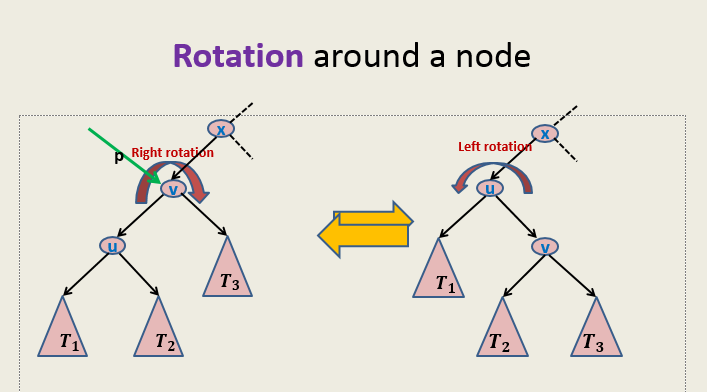
\includegraphics[scale=0.5]{fig1.png}
\caption{Rotation}
\label{fig1}
\end{figure}
\begin{itemize}
\item During Rotation, only 2 nodes are affected and rest of the subtree's fields will remain the same as shown in figure-\ref{fig1}.To update their values, update function is called for the 2 nodes u and v. Hence it takes $O(1)$ time.
\end{itemize}
\item \textbf{MaxOverlap:}	
\begin{itemize}
\item At any node v, the Augmented field pointMax(v) stores the point with maximum overlap in the subtree of v. Therefore pointMax(ROOT) will give the point with maximum overlap in the entire interval tree.
This can be achieved in $O(1)$ time.
\end{itemize}

\end{itemize}


\end{document}